\documentclass{article}

\usepackage{lipsum}
\usepackage[margin=1in,includefoot]{geometry}
\usepackage{graphicx}
\usepackage{float}
\usepackage[hidelinks]{hyperref}
\usepackage{amsmath}
\usepackage{amssymb}

% Header and Footer Stuff
\usepackage{fancyhdr}
\pagestyle{fancy}
\fancyhead{}
\fancyfoot{}
\fancyfoot[R]{\thepage}
\renewcommand{\headrulewidth}{0pt}
\renewcommand{\footrulewidth}{0pt}

\begin{document}

\begin{titlepage}
	\begin{center}
	\begin{align*}
	
\includegraphics[height=1.75in]{logo.png}
	\end{align*}


	
	\line(1,0){300}\\
	[0.25in]
	\huge{\bfseries Film Q}\\
	[2mm]
	\line(1,0){200}\\
	[1.5cm]
	\textsc{\LARGE Android Project}\\
	[0.75cm]
	\textsc{\Large 3D5B Software Design and Implementation}\\
	[7cm]	
	\end{center}
	
	
	
	\begin{flushright}
	\textsc{\large Alexandru Sulea\\
	D Stream\\
	\#12315152\\
	8 January 2016\\}
	\end{flushright}

\end{titlepage}



\thispagestyle{empty}
\cleardoublepage
\pagenumbering{arabic}
\setcounter{page}{1}


\section{Introduction}\label{sec:intro}
The purpose of this project is to explore the design and development cycle of an android app. In this project the concepts of large group work and a standardized development platform will be explored and implemented to see if a functional android app can be produced within the allotted time.\\
 The project is designed to not only test the design and coding  skills of the group but also the planning and team work aspect as well.

\section{Theory}\label{sec:theory}
The concept for our android project revolved around developing a movie based quiz.
Upon opening the application 3 list options would be populated on the main screen. The data from these options would be automatically scraped using a JSON scrapper from the unofficial imdb API. 
The user would have 3 options:
First option would be a Plot quiz. Upon choosing the plot quiz the user would be confronted with a short abbreviated quiz from a movie and be given 4 options of movie titles , one which would be correct option regarding the movie title.\\
The second option would be to choose the random actors quiz, here the user would be again confronted by the same type of set-up. Only this time the user would be given a random movie title with a random character name from that movie. The user would be given 4 options of actors names and would have to choose the correct actor name.\\
The third and last option would be to select a movie from a list view. The list view itself would be populated by data scrapped from the imdb API of the top 250 movies. Upon entering the quiz the user will be confronted by a random character name and four actor names. The user would have to choose the correct actor name form the given options. \\
The quiz is time based. Upon starting the quiz the user is given 16 seconds to complete the quiz. If a wrong answer is selected the quiz will rotate to the next question with the timer still decreasing to zero. If the correct answer is selected the timer will increase by 5 seconds and  will rotate to the next question. \\
Upon completion of the quiz the high score will be calculated by taking into account the number of correct answers given the number of questions attempted within the relevant time range. The higher scores will be given to the user who had the the most correct answers within the longest amount of time.\\
When the quiz is completed the user will be confronted with four more options. The options are to go back replay the same quiz again and see if they can beat their own high score.To return home. To share the result on Facebook or to register the high score online.\\
The last option is especially important. Upon selecting to register the high score. The user will be confronted by an old time arcade name input interface. After entering their name the high score will be stored in an Amazon server for all the other players to view and of course try to defeat.\\



\pagebreak
\section{Results}\label{sec:result}

\begin{align*}
\centering
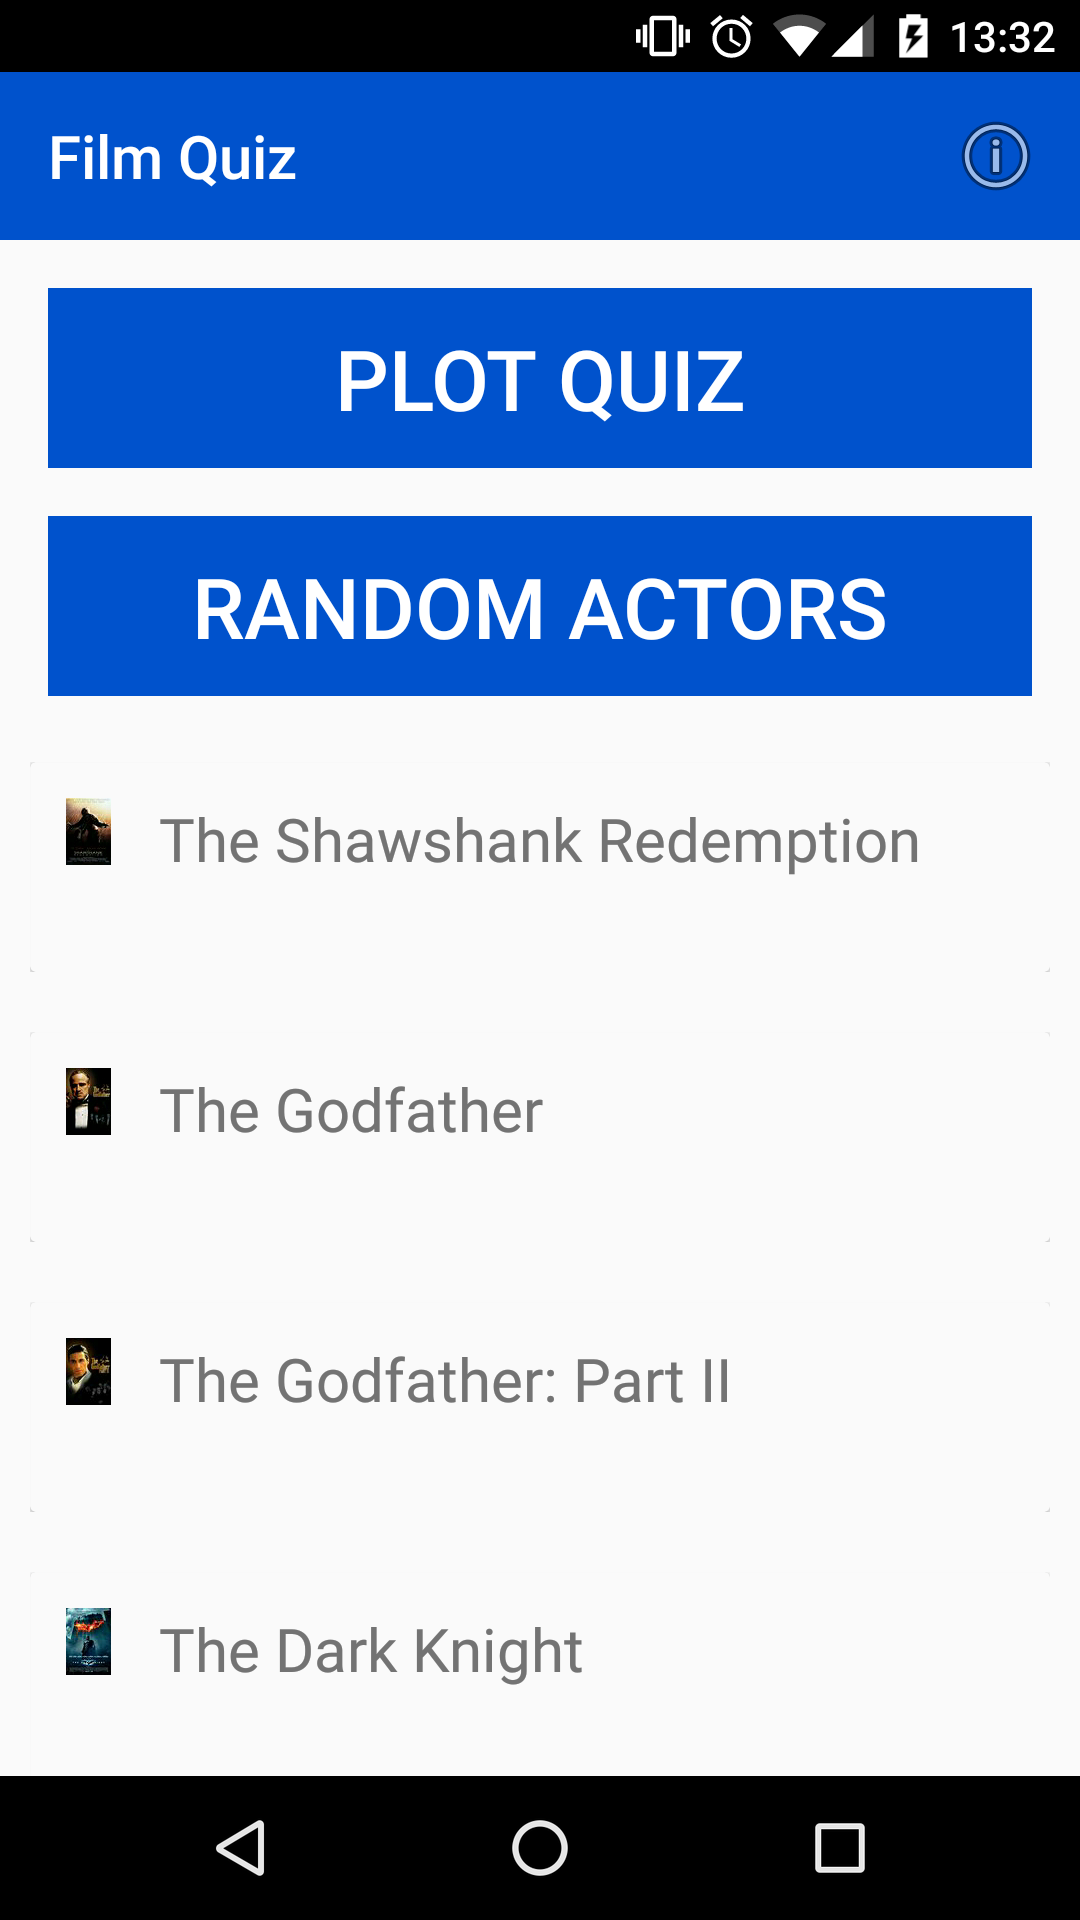
\includegraphics[height=3.75in]{s1.png}
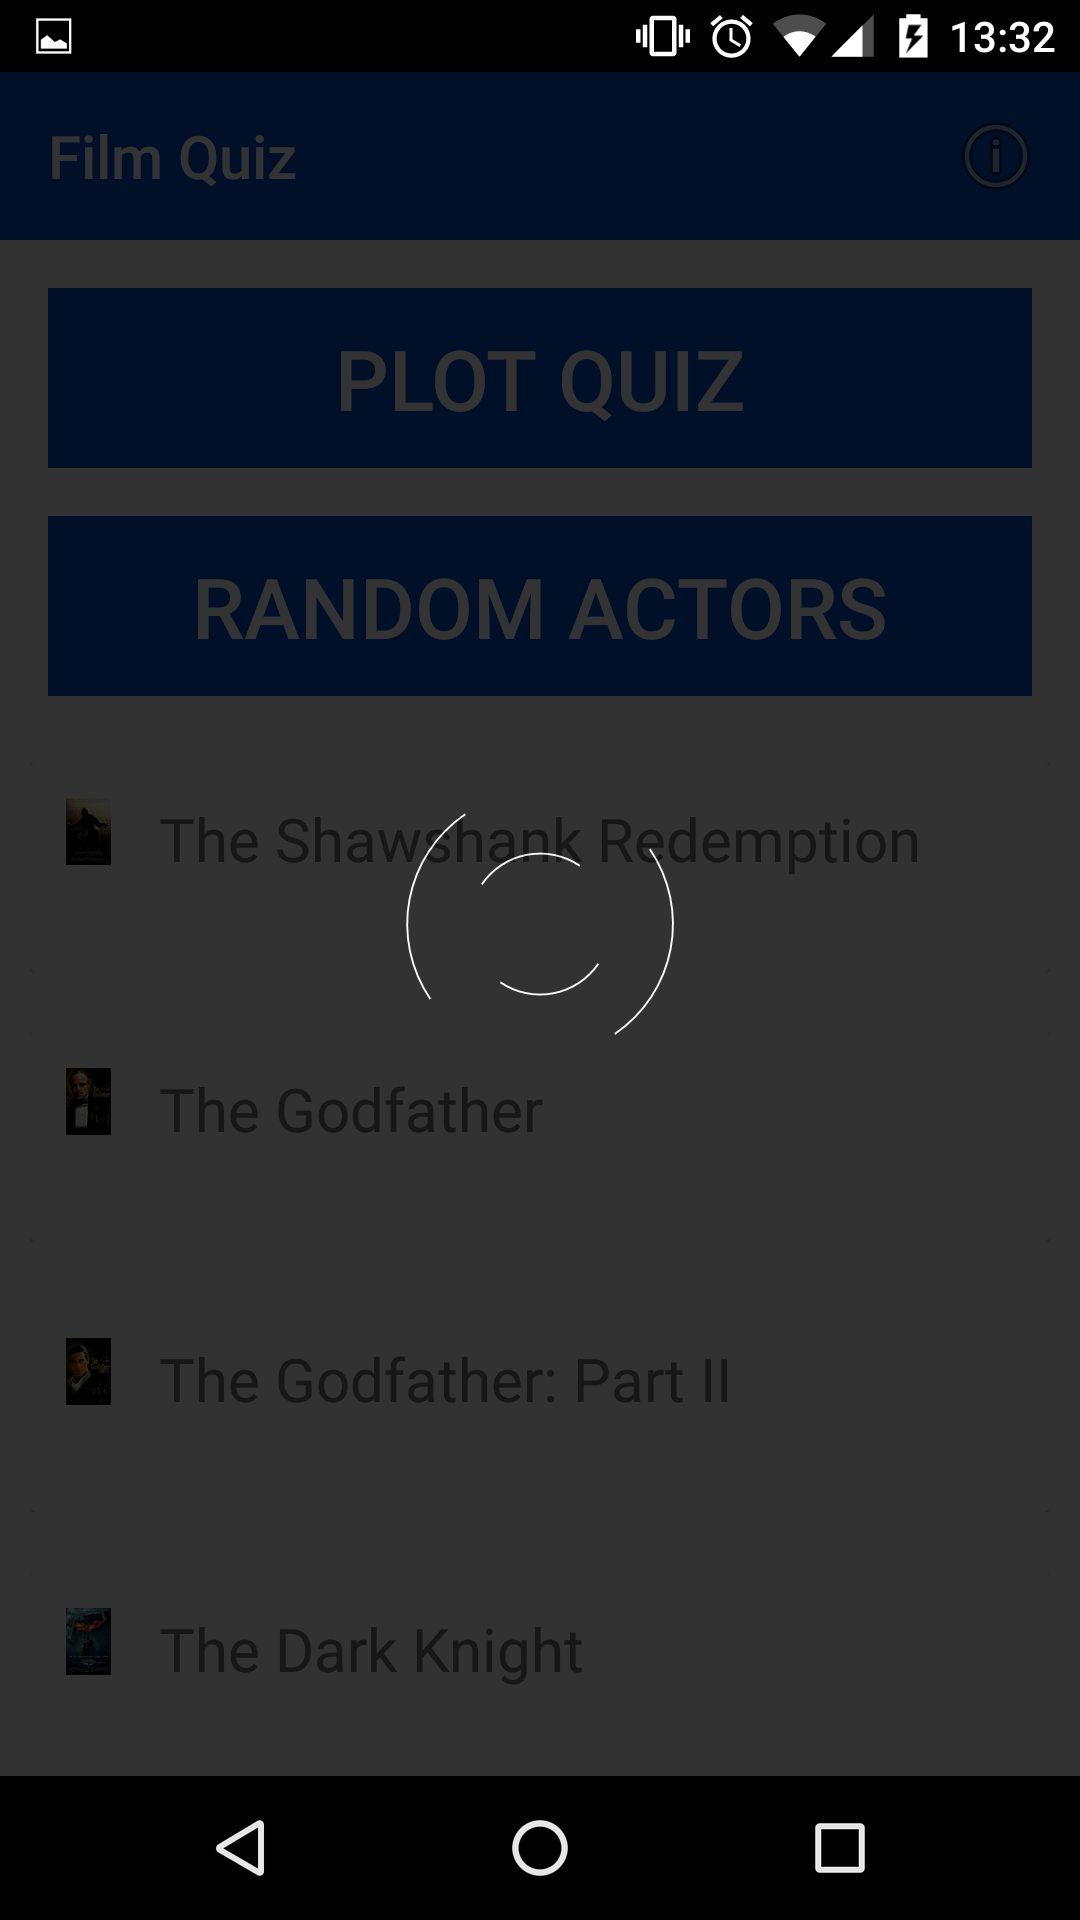
\includegraphics[height=3.75in]{s2.png}
\end{align*}\\



\begin{align*}
\centering
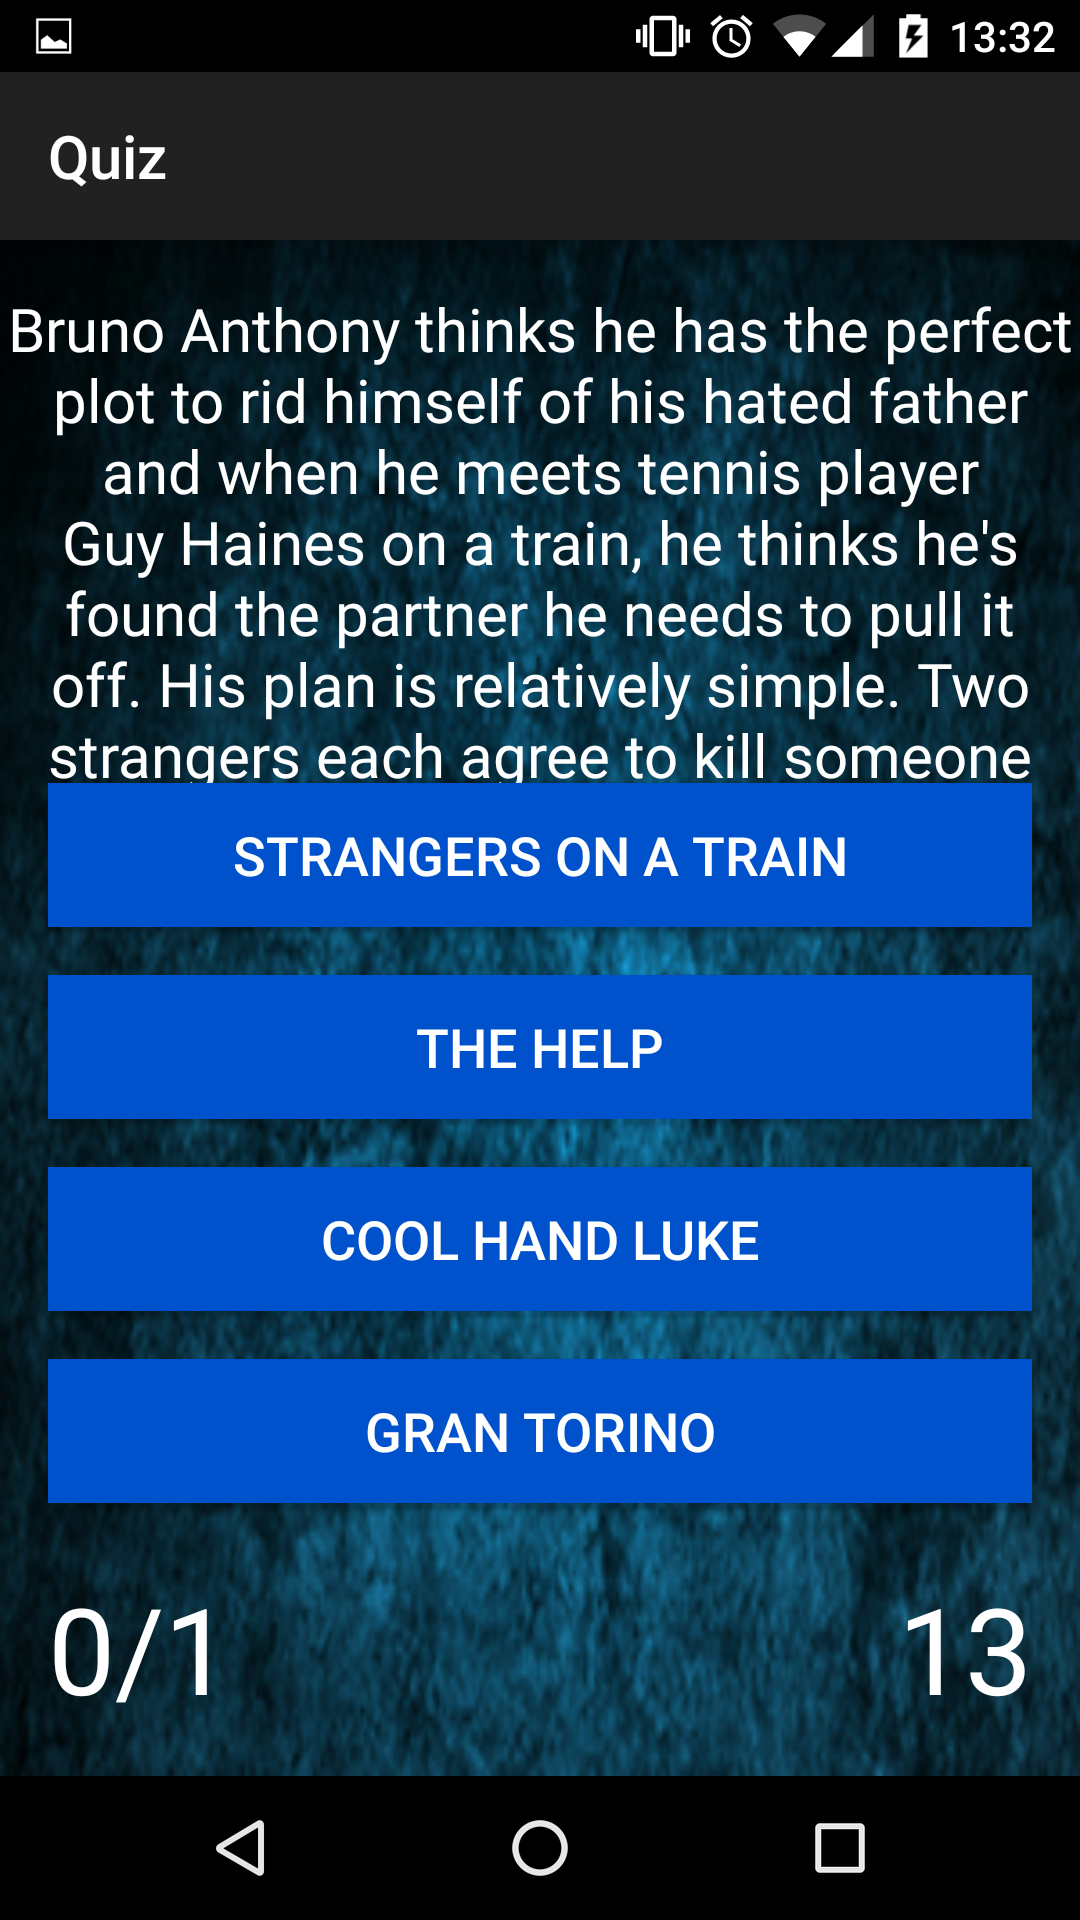
\includegraphics[height=3.75in]{s3.png}
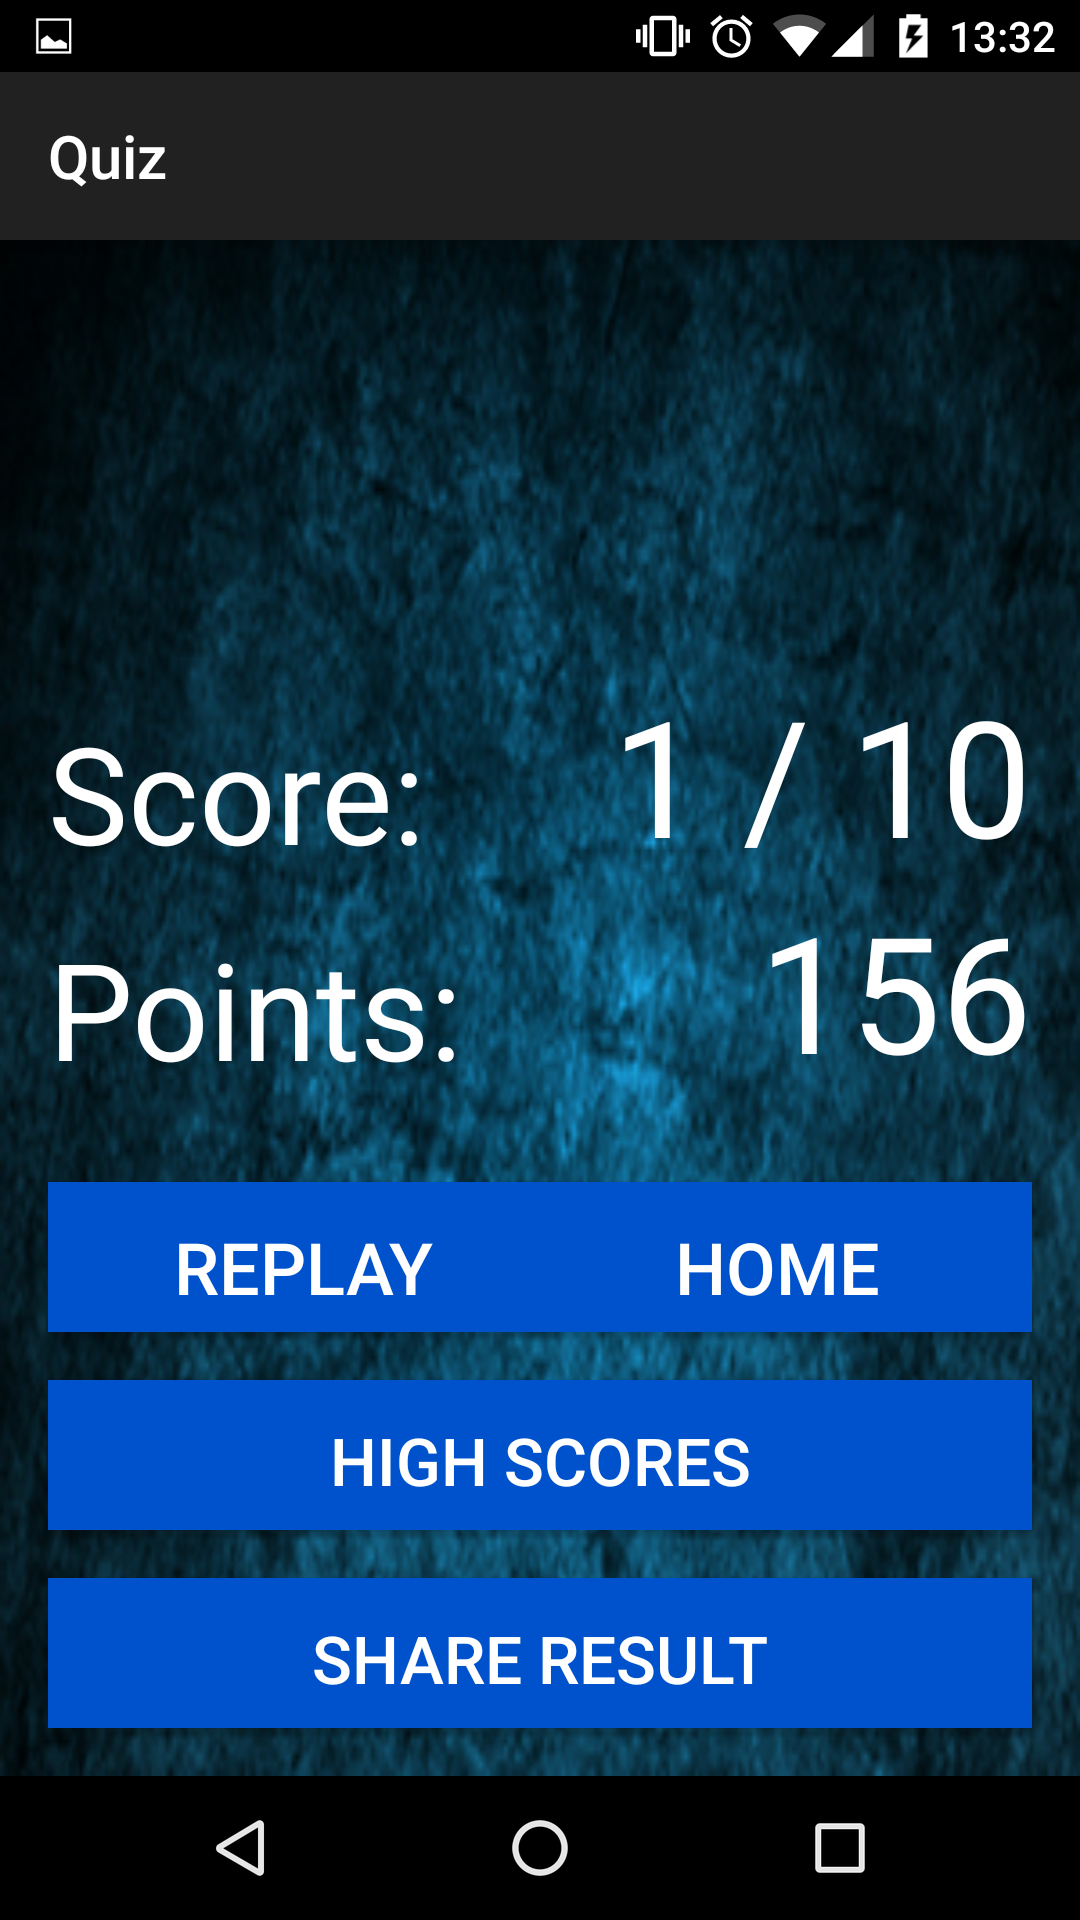
\includegraphics[height=3.75in]{s4.png}
\end{align*}\\


\begin{align*}
\centering
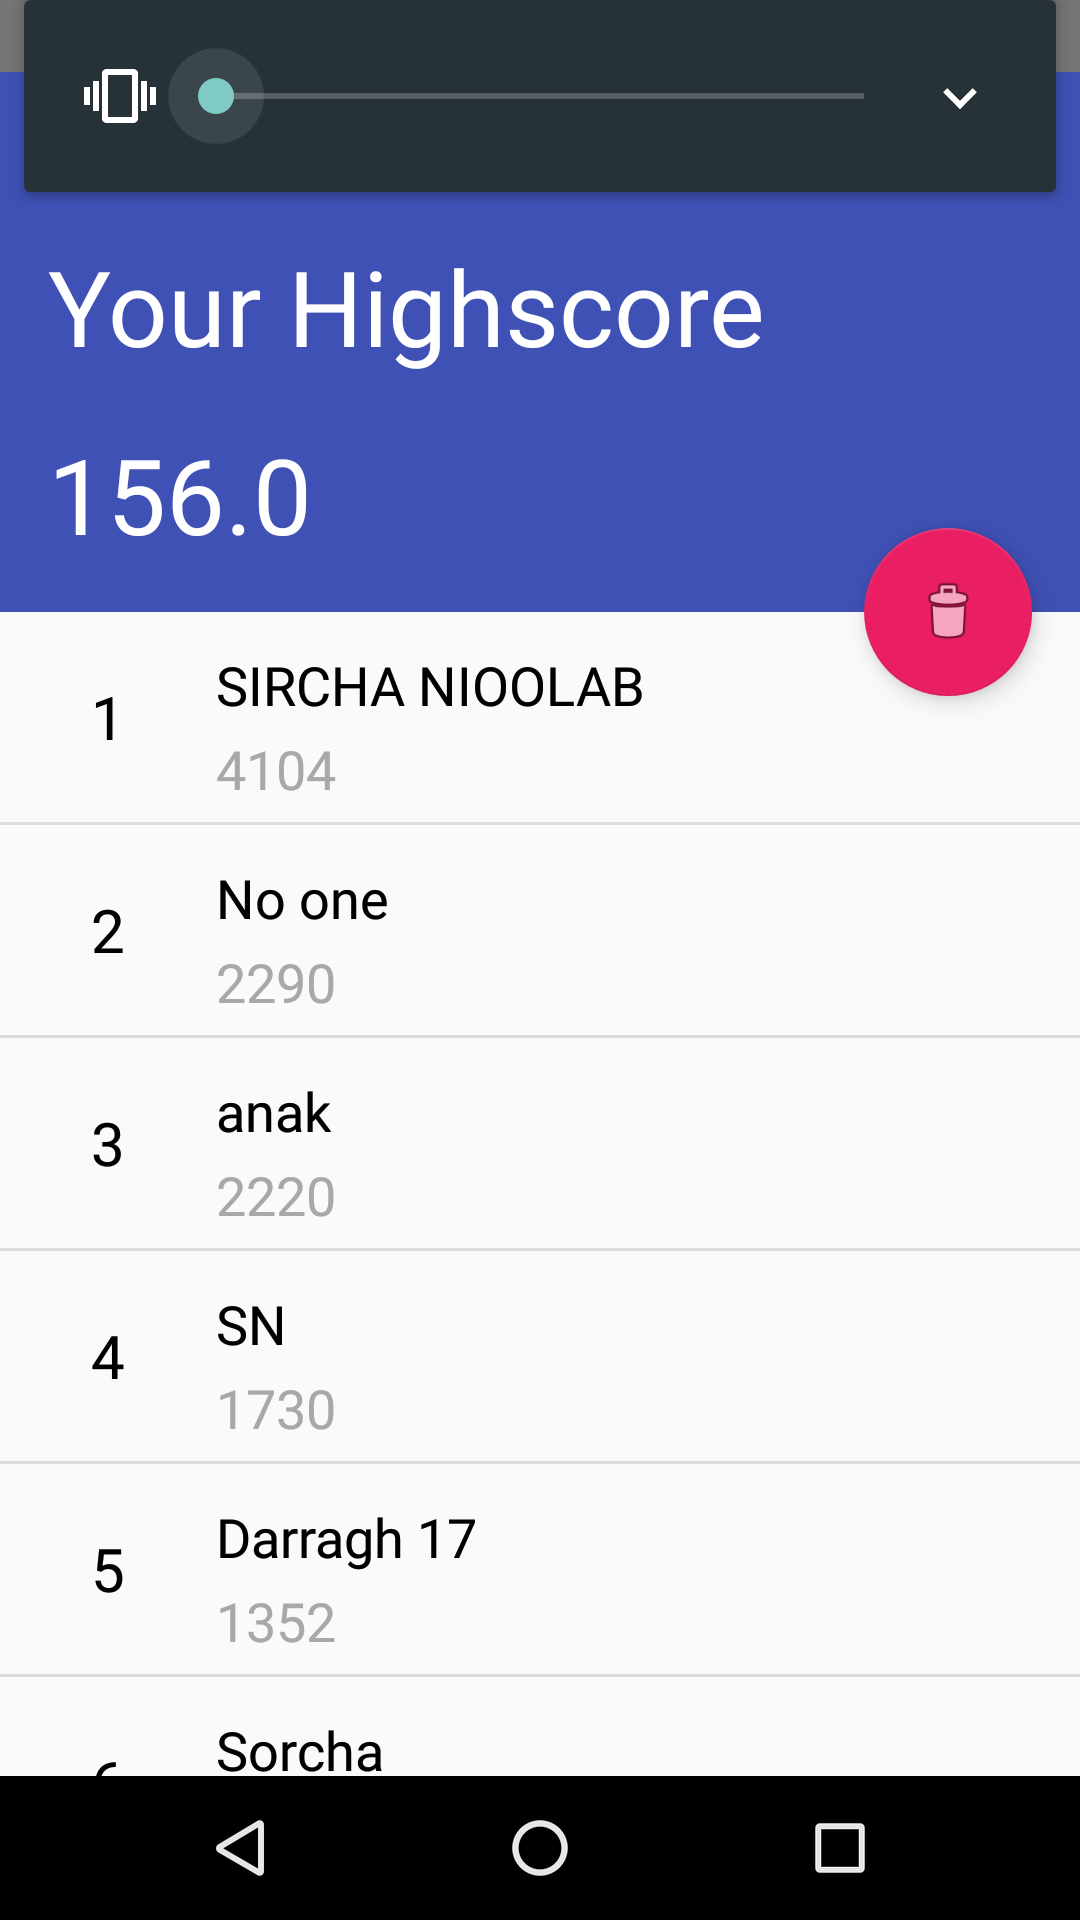
\includegraphics[height=3.5in]{s5.png}
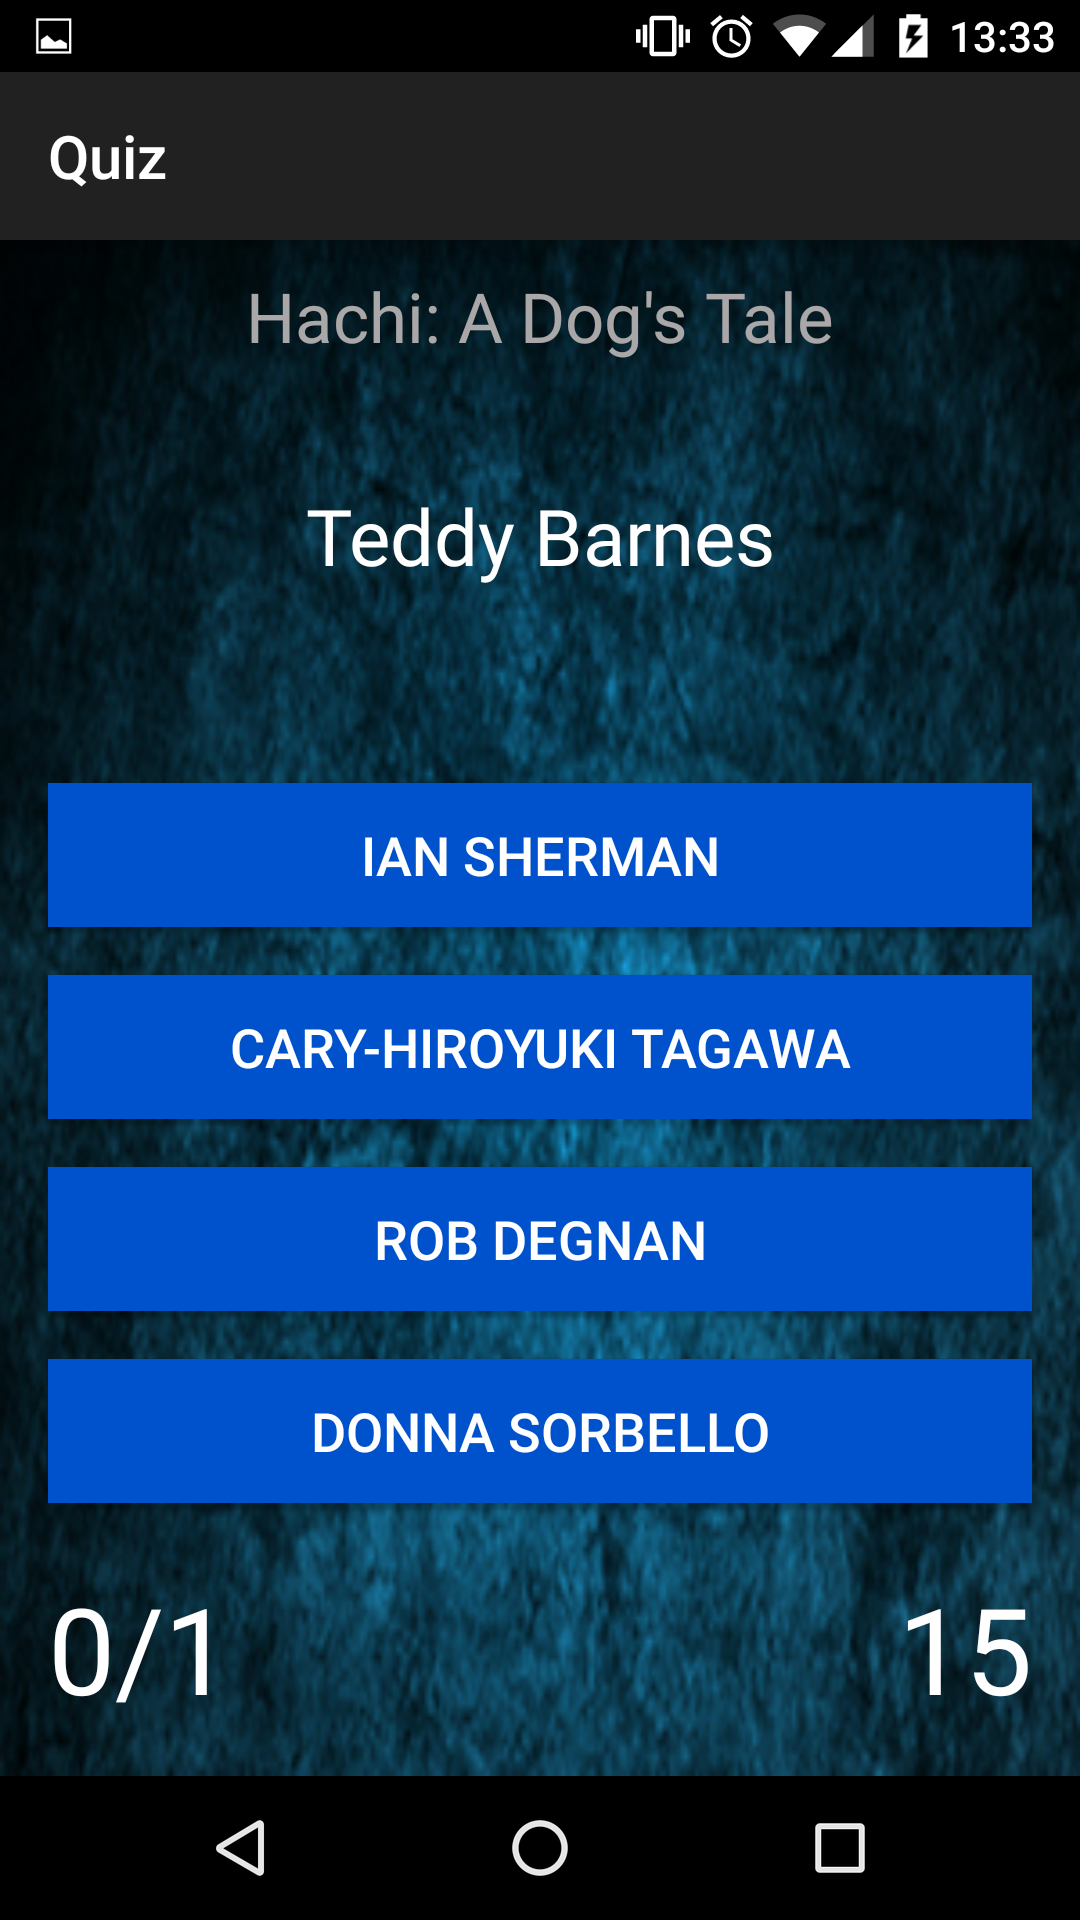
\includegraphics[height=3.5in]{s6.png}
\end{align*}\\

\begin{align*}
\centering
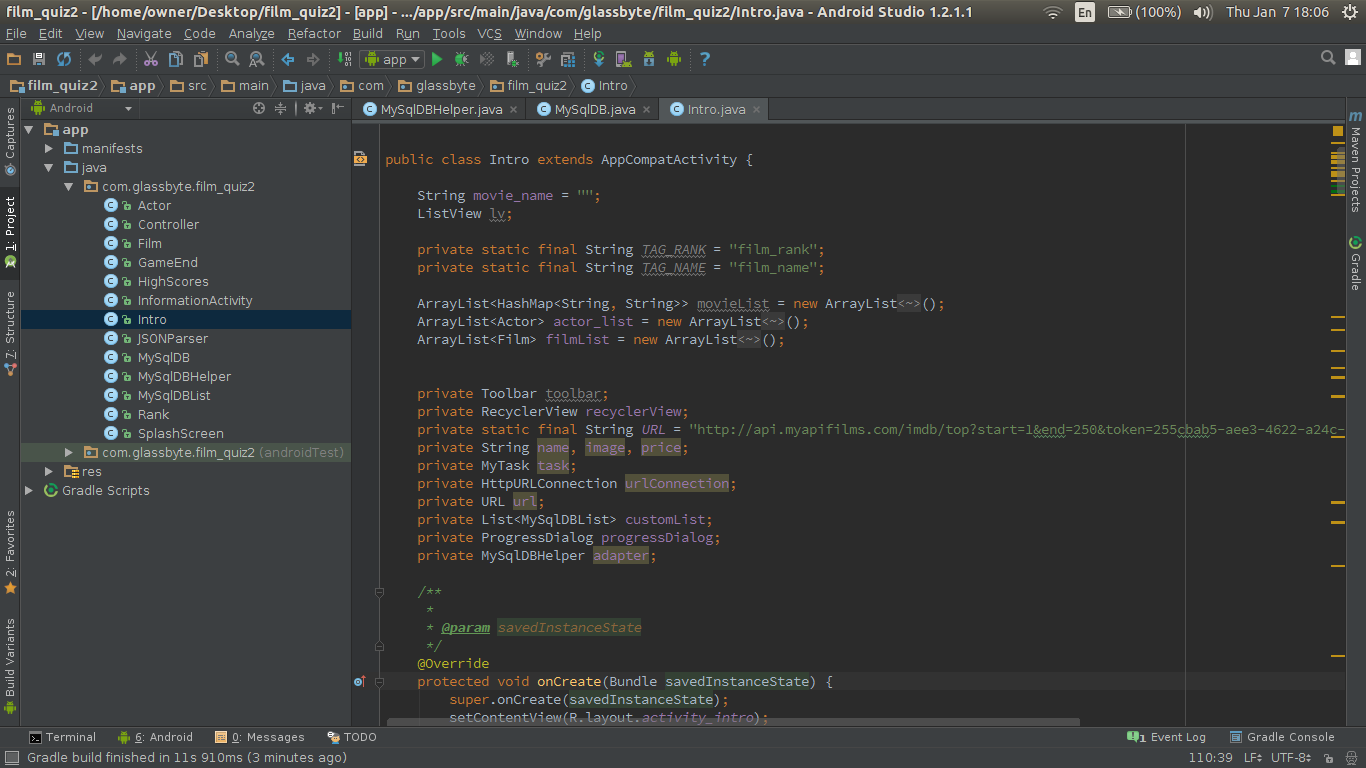
\includegraphics[height=3.5in]{s7.png}
\end{align*}\\

\begin{align*}
\centering
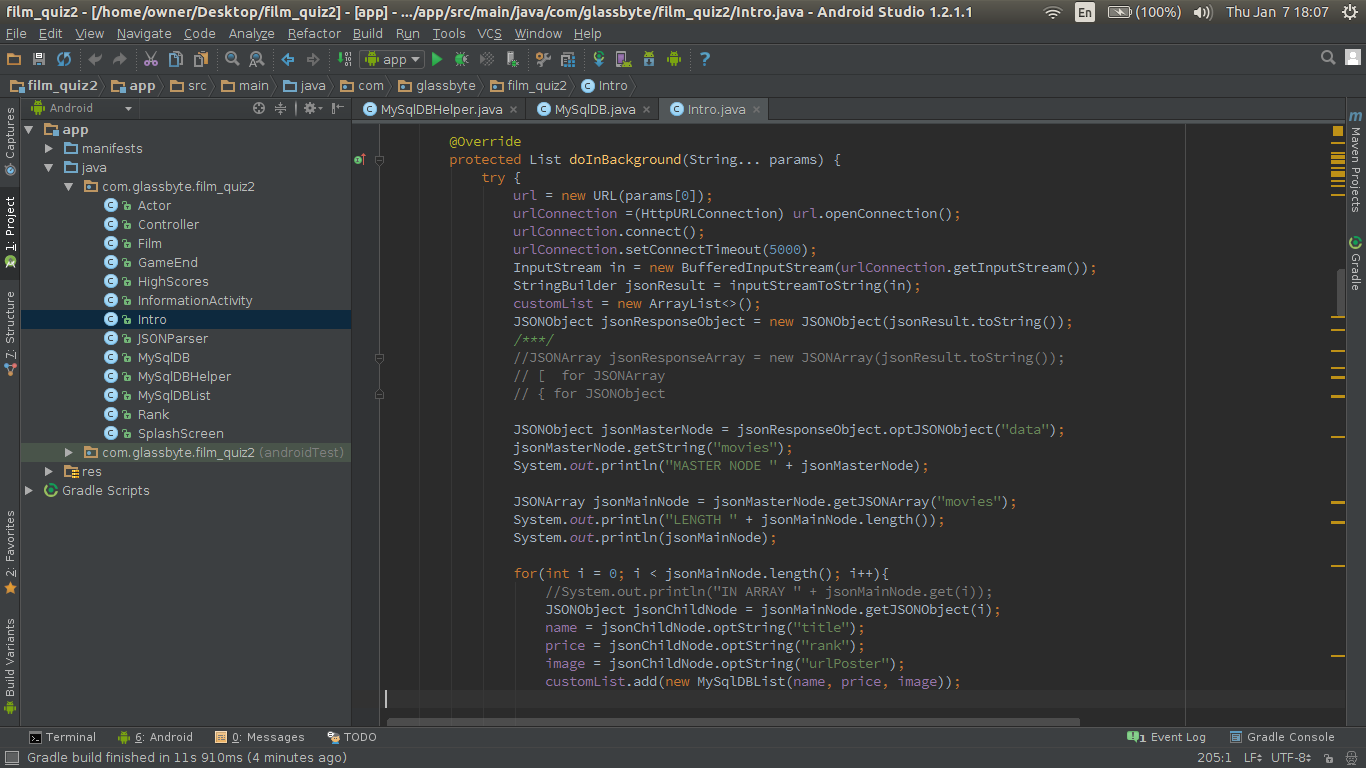
\includegraphics[height=3.5in]{s8.png}
\end{align*}\\

\begin{align*}
\centering
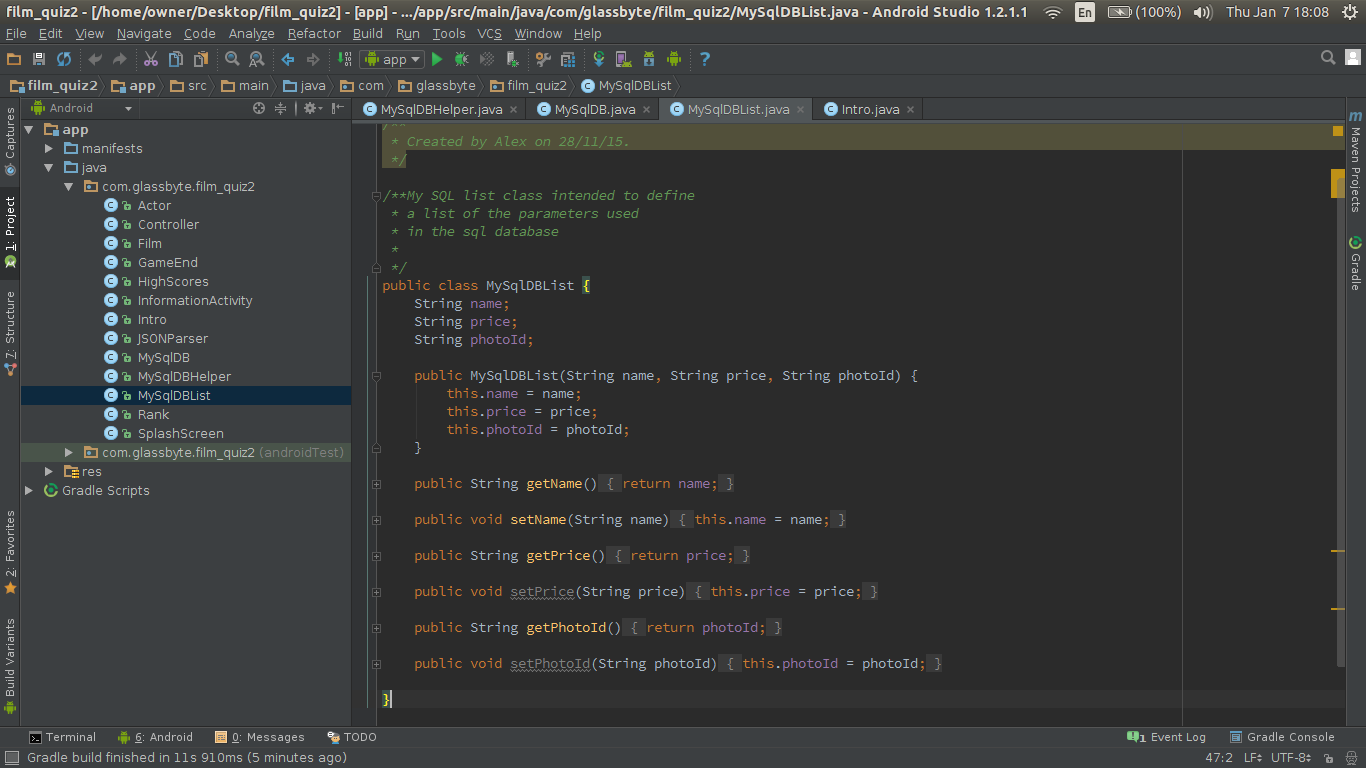
\includegraphics[height=3.5in]{s9.png}
\end{align*}\\



\begin{flushleft}
\section{Discussion}
The project was already past concept phase when I joined the group. The group had already divided the jobs among themselves thus I was left with whatever parts were not finished or assigned yet.\\
My part was thus comprised of parsing the unofficial imdb API correctly. Setting up an .xml display view such as  a list view display and then inputting the parsed data correctly into the respective classes handling the various quiz options.\\
Since nothing was set up in that respect, I set about trying to make a mySQL database to handle the data after it is being parsed. Due to time constraints however I was not able to implement the mySQL database and thus the classes handling the parsing of JSON data are somewhat mislabeled as mySqlDB.\\
Although the classes are mislabeled the JSON parser fully works and correctly links data into the appropriate displays.\\ 
My specific contributions to the project are in MySqlDB, MySqlDBHelper, MySqlDBList and the JSON parsing and Asynchronous control parts of Intro activity which is our projects ".MainACtivity" .These activities only parse the 250 most popular movie names along with the pictures and ranking, the parsing of the actor names is handled in a different activity created by Darragh. On the display side they include the dynamic list view with cardboard individual slots which can also display the parsed pictures.(Please see above pictures for details)\\
Challenges:\\
1. Parsing the JSON data properly, due to the fact that JSON has arrays within objects which can contain other objects with arrays in them. It was important to have a good understanding of how data can be formatted so as to parse it correctly.\\
2. Gradle Errors.\\
3. Making sure to stick to a specific time table of when everyone can add their parts to the main activity so as to avoid merge confrontations.\\
Solutions:\\
1. Read about JSON parsing and attempted a few simple small examples before proceeding to implement the film quiz parsing activities.
2. Could not resolve the gradle errors. Had to start a new project altogether. The code was copied over manually to the new Android Project.\\
3. Used the meeting time to establish a time table for when to add our specific parts,(if pushing to the same activity)  so as to avoid merge conflicts.\\
Team:\\
In my opinion the team was very well managed, and we have hit all of our intended goals as far as the technical side of the project is concerned. Due to the fact that we had weekly and towards the end, bi-weekly meetings, team communication was very good and we were able to work consistently and quickly to finish the project.\\

\end{flushleft}



\section{Conclusion}
The project proved somewhat challenging from a coding point of view due to the fact that I have never attempted to parse data using JSON.\\
The second challenging aspect was the unofficial imdb API itself. Due to some data errors. There ware many missing data parts from some pages in the imdb API. Overcoming these unintended and unforeseen setbacks was an important learning lesson.

\pagebreak

\section{Grading}
$$\textbf{Team Members}$$
$$Sarah ---1$$
$$Darragh ---2$$
$$Robby ---3$$
$$Cian ---4$$
$$Sorcha ---5$$

$$\textbf{APPS}$$
$$FilmQ ---1$$
$$Casper ---2$$
$$To do List ---3$$
$$SpaceShare ---4$$
$$Cheecky checks ---5$$
$$Morse ---6$$
$$College Calendar ---7$$

\end{document}